\documentclass[11pt,a4paper]{article}
\usepackage[margin=2.2cm]{geometry}
\usepackage[T1]{fontenc}
\usepackage{lmodern}
\usepackage{microtype}
\usepackage{amsmath,amssymb,amsthm}
\usepackage{booktabs}
\usepackage{graphicx}
\usepackage{xcolor}
\usepackage{listings}
\usepackage{hyperref}
\usepackage{setspace}
\onehalfspacing
\graphicspath{{figures/}}

% Red marker for numbers that must be filled in / checked against results/*.csv
\newcommand{\todo}[1]{\textcolor{red}{[\textbf{CHECK:} #1]}}
\newtheorem{proposition}{Proposition}
\lstset{basicstyle=\ttfamily\small,breaklines=true,frame=single,columns=fullflexible}

\title{Where Does the Cost of Bounds Checking Go?\\
Check Encoding, Dispatch Technique, and ISA-Preserving Loop-Guard Hoisting\\
in a Stack-Based Virtual Machine}
\author{Abhiram \\
Department of Computer Science and Engineering (Data Science)\\
Vellore Institute of Technology, Vellore, India\\
\texttt{[email]}}
\date{}

\begin{document}
\maketitle

\begin{abstract}
Array bounds checks are the standard price of memory safety in virtual machines (VMs), and compile-time analysis is the standard way to avoid paying it. In a bytecode interpreter the cost of a check has two parts that are usually conflated: the comparison, and the extra bytecode that must be fetched and dispatched to perform it. We study how these parts behave on a complete from-scratch toolchain: a small imperative language (MiniL), a compiler with interval abstract interpretation, and a stack VM with three dispatch implementations (\texttt{switch}, computed goto, direct threading). The compiler emits several encodings of the same program: unchecked (U), separate check instructions (R), fused checked accesses (F), interval-based elimination (S), elimination plus an ISA-preserving loop-guard hoisting pass (H), and combinations of fusion with elimination (FS, FH). Two experimental modes isolate dispatch from comparison: N dispatches an extra do-nothing instruction, and FN fuses the access but omits the comparison. On a suite of 22 array benchmarks, separate checks cost only $+2.16\%$ in geometric-mean time under computed goto, but the overhead depends strongly on the dispatch technique ($+5.32\%$ with \texttt{switch}, $+0.32\%$ with direct threading). The extra dispatch alone (mode N) accounts for about half of the separate-check cost under computed goto and over $80\%$ under \texttt{switch}. Fusing the check helps under \texttt{switch} ($-2.41\%$) but not under computed goto ($+3.49\%$), so ``fuse the check'' is not a universal remedy. Interval analysis removes $77.9\%$ of static access sites' checks and, with hoisting, $88.5\%$ of dynamic checks, reducing overhead to $+0.69\%$ without adding any opcode to the VM. A fault-injection study with 213 faulty mutants shows that $91.5\%$ raise new static alarms, while unchecked execution never crashed and ran silently on $85.0\%$. We present an applied, reproducible measurement study; the interval domain and loop versioning are classical, and our contribution is the controlled decomposition across encodings and dispatch styles and the ISA-preserving formulation of the guard.
\end{abstract}

\noindent\textbf{Keywords:} bounds checking, virtual machines, interpreter dispatch, abstract interpretation, check elimination, loop versioning, fault injection.

%--------------------------------------------------------------------
\section{Introduction}
Memory-safe execution requires that every array access be either proven or checked to lie within its object. Managed runtimes, smart-contract platforms and WebAssembly engines all enforce this, and the cost of doing so has been studied extensively for native and JIT-compiled code~\cite{haas2017,jangda2019,nagarakatte2009,serebryany2012,akritidis2009}. Two families of remedies exist: make the check cheaper, or make it unnecessary by proving it redundant at compile time~\cite{suzuki1977,gupta1993,kolte1995,bodik2000,midkiff1998,wurthinger2009}.

Both remedies are usually evaluated under a native-code cost model in which a check is a compare and a well-predicted branch. A bytecode interpreter has a different cost structure. Each executed VM instruction pays a dispatch cost that was historically attributed to indirect-branch misprediction~\cite{proebsting1995,ertl2003,casey2007}, although modern predictors have changed this picture~\cite{rohou2015}, and instruction-pointer update dependencies remain relevant~\cite{ertl2024}. If a check is encoded as a separate instruction, its cost therefore includes a dispatch that has nothing to do with the comparison it performs. This suggests the benefit of eliminating checks, and of cheaper encodings such as fusing the check into the access opcode, depends on how the VM dispatches.

We test this on a controlled, fully reproducible stack of our own, so that the encoding of the check, the dispatch technique and the analysis can each be varied independently.

\paragraph{Research questions.}
\begin{itemize}
\item \textbf{RQ1} What is the overhead of bounds checking in a stack VM, and how does it depend on the dispatch technique?
\item \textbf{RQ2} How much of that overhead is due to dispatching an extra instruction rather than performing the comparison?
\item \textbf{RQ3} What fraction of checks can be eliminated at compile time (statically and dynamically), and how much overhead does that recover, including with a loop-guard hoisting pass that needs no new VM opcode?
\item \textbf{RQ4} Which faults does static analysis notice, and which must remain runtime checks?
\end{itemize}

\paragraph{Contributions.} Interval analysis and loop versioning are classical and we claim no new abstract domain. Our contributions are:
\begin{enumerate}
\item A controlled \emph{encoding $\times$ dispatch} study of bounds-check cost in an interpreter, including two synthetic modes (N and FN) that separate the cost of the extra dispatch from the cost of the comparison (Sections~\ref{sec:method} and~\ref{sec:results}).
\item An \emph{ISA-preserving} formulation of loop-guard hoisting: the loop-entry guard is compiled to ordinary arithmetic and conditional jumps, so the trusted VM is unchanged (Section~\ref{sec:hoist}).
\item A negative-result-aware evaluation: we report that fused checks are not uniformly beneficial, that overheads are small and near the noise floor on our platform, and that conclusions depend on dispatch style.
\item A reproducible protocol (paired, interleaved timing with bootstrap confidence intervals, a null-control benchmark, mutation-based fault injection and differential testing across all checked modes), with all code, data and scripts released with the paper.
\end{enumerate}

%--------------------------------------------------------------------
\section{Background and Related Work}
\paragraph{Check elimination.} Suzuki and Ishihata described one of the earliest array-bound checkers based on static assertions~\cite{suzuki1977}. Gupta moved checks out of loops using flow analysis~\cite{gupta1993}, Kolte and Wolfe organised checks into implication families to remove redundant ones~\cite{kolte1995}, and ABCD performs demand-driven elimination over an inequality graph~\cite{bodik2000}. Midkiff, Moreira and Snir applied loop versioning to Java array references~\cite{midkiff1998}. W\"urthinger et al.\ combined a fast analysis with deoptimization in the HotSpot client compiler~\cite{wurthinger2009}. Our analysis is deliberately simpler (non-relational intervals with condition refinement), because our aim is to quantify effects in an interpreter, not to improve precision. Relational domains such as polyhedra~\cite{cousot1978} and octagons~\cite{mine2006} would prove strictly more.

\paragraph{Verifier-style bounds reasoning.} The Linux eBPF verifier is a close relative of our guard-based approach: it contains no dedicated bounds-check instruction, and instead tracks value ranges through ordinary conditional jumps, accepting accesses whose ranges it can prove safe~\cite{vishwanathan2023}. The difference is when the reasoning happens. The verifier rejects or accepts a program statically, whereas our compiled guard is evaluated at run time and selects between an unchecked and a fully checked version of the same loop.

\paragraph{Interpreter dispatch and superinstructions.} Proebsting showed that interpreter speed is dominated by dispatch and proposed superoperators that merge instruction sequences~\cite{proebsting1995}. Ertl and Gregg studied the interaction of dispatch with branch prediction~\cite{ertl2003,casey2007}, and Rohou et al.\ argued that on modern hardware this folklore needs revisiting~\cite{rohou2015}. Ertl and Paysan examine the cost of instruction-pointer updates~\cite{ertl2024}. Stack versus register VM design has been compared by Shi et al.~\cite{shi2008}. A fused checked access is the stack-VM analogue of a superinstruction.

\paragraph{Cost of safety.} WebAssembly relies on bounds checks and its overhead against native code has been analysed in detail~\cite{haas2017,jangda2019}. C-level spatial safety systems report overheads that depend on their metadata scheme~\cite{nagarakatte2009,serebryany2012,akritidis2009,necula2005,jones1997}. In contrast to these native-code studies, we measure a bytecode interpreter, where the encoding of the check interacts with dispatch. To our knowledge no earlier study isolates the dispatch component of a bounds check in an interpreter with a controlled decomposition, but we have not performed an exhaustive literature search.

\paragraph{Verification.} Verified compilation~\cite{leroy2009} offers the strongest assurance that transformations preserve behaviour; we instead validate preservation empirically by differential testing and by a randomized soundness test.

%--------------------------------------------------------------------
\section{System Design}\label{sec:design}
\subsection{Language and toolchain}
MiniL is a small imperative language with 64-bit signed integer scalars, global fixed-size integer arrays, assignment, \texttt{if/else}, \texttt{while}, \texttt{return}, \texttt{print}, and functions with integer parameters, locals and recursion. Division and remainder follow C semantics (truncation). The compiler is written in Python 3 using only the standard library and consists of a lexer, a recursive-descent parser producing an AST in which every array access carries a unique \emph{site identifier}, a semantic pass (name resolution, arity checks, frame-slot allocation), a static safety analysis (interval analysis and hoisting planner), and a code generator parameterised by mode. A statically definite violation never changes the emitted code: it is reported as a compile-time diagnostic and the access is still checked, so all checked modes trap identically.

\subsection{Stack VM and instruction set}
The VM is written in C11 and executes fixed-size three-word instructions (opcode, operands $a$ and $b$) over an operand stack, a call stack with frame-relative \texttt{LOAD}/\texttt{STORE}, and a flat memory in which arrays are contiguous. Memory is padded between and after arrays so that moderate unchecked out-of-bounds accesses corrupt neighbouring data silently, as in real unchecked runtimes. The instruction set comprises \texttt{PUSH}, \texttt{LOAD}, \texttt{STORE}, arithmetic and comparison operators, \texttt{JMP/JZ/JNZ}, \texttt{CALL/ENTER/RET}, \texttt{PRINT}, \texttt{HALT}, the unchecked \texttt{ALOAD/ASTORE}, the separate check \texttt{CHK a}, which traps unless $0\le \text{top}<|a|$ using a single unsigned comparison and does not pop its operand, and the fused \texttt{ALOADC/ASTOREC}, which perform the same check and the access in one dispatch. A trap terminates with a distinct exit status and a message naming the array and the source access site. The full opcode table is in the repository (\texttt{docs/isa.md}).

\paragraph{Dispatch.} The dispatch technique is selected at compile time. \texttt{SWITCH} uses a C \texttt{switch} in a loop; \texttt{GOTO} uses GCC computed goto with one indirect jump per handler; \texttt{DIRECT} is direct-threaded, with handler addresses resolved in the instruction stream before execution. We additionally build the GOTO interpreter with \texttt{-O3} (\texttt{OPT3}). The VM measures the wall-clock time of the interpreter loop only (monotonic clock, excluding start-up and bytecode loading), and a \texttt{-DCOUNT} build counts executed instructions and checks.

\subsection{Compilation modes}
Table~\ref{tab:modes} lists the modes. U, R, F, S and H correspond to the base design; FS and FH combine fusion with elimination, so that fused checks are used only at sites that could not be proven safe. N and FN exist only to decompose cost: they use experimental opcodes compiled under a separate build flag and are \emph{outside} the trusted-ISA claim.

\begin{table}[t]
\centering
\caption{Compilation modes.}\label{tab:modes}
\small
\begin{tabular}{@{}lp{11.5cm}@{}}
\toprule
Mode & Check emission policy \\
\midrule
U & No checks (fast, unsafe). \\
R & \texttt{CHK} before every \texttt{ALOAD/ASTORE} (explicit-check encoding). \\
F & \texttt{ALOADC/ASTOREC} at every access (same checks, no extra dispatch). \\
S & As R, but \texttt{CHK} omitted at sites proven safe by interval analysis. \\
H & As S, plus loop-guard hoisting (Section~\ref{sec:hoist}). \\
FS & Fused access only at sites not proven safe; plain access where proven. \\
FH & As FS, plus hoisting; the fallback loop uses fused checks. \\
N & As U, plus a do-nothing \texttt{NOPCHK} dispatched before every access (extra dispatch, no comparison). \\
FN & Fused-style opcode with the comparison removed (opcode fusion without check cost). \\
\bottomrule
\end{tabular}
\end{table}

\subsection{Interval analysis}
For each function we run a forward abstract interpretation over the AST with the non-relational interval domain $I=\{[l,h]\mid l\le h\}\cup\{\bot\}$ extended with $\pm\infty$, mapping each integer variable to an interval. Parameters and values loaded from arrays are $\top$. Arithmetic uses standard interval transfer functions with truncating division and C-style remainder (for an unknown signed $x$, $x\bmod 64\in[-63,63]$). Branch and loop conditions refine the state: for a relation $x+k \bowtie e$ the interval of $x$ is intersected with the interval of $e$ shifted by $-k$, and symmetrically for the right operand, so that, for example, $j<N-1-i$ with $i\in[0,N-2]$ yields $j\le N-3$. Loops are solved by Kleene iteration with widening after two iterations followed by two narrowing steps. A final recording pass joins, for every access site $s$ into array $a$, the interval $I_s$ of its index, and classifies the site:
\[
\mathrm{class}(s)=\begin{cases}
\textit{safe} & I_s\subseteq[0,|a|-1]\\
\textit{violation} & I_s\cap[0,|a|-1]=\emptyset\\
\textit{unknown} & \text{otherwise.}
\end{cases}
\]
Under the assumption that integer arithmetic does not wrap (not modelled; documented in the repository), safe sites cannot go out of bounds in any execution, and violation sites always do if reached. Soundness follows the standard argument~\cite{cousot1977}; we also test it empirically with a randomized test that generates many well-formed programs, runs them under R, and asserts that no site classified safe ever traps.

\subsection{ISA-preserving loop-guard hoisting}\label{sec:hoist}
Interval analysis cannot prove accesses whose bound is a run-time parameter, for example \texttt{while (i < m) \{ s = s + a[i]; i = i + 1; \}} with $m$ unknown. Yet a single test before the loop suffices. The planner considers every \emph{innermost} loop of the form
\begin{equation}
\texttt{while (i}\ \lhd\ E\texttt{) \{ \dots; i = i + c \}},\qquad \lhd\in\{<,\le\},\ c\ge 1,\label{eq:loop}
\end{equation}
where the increment is the last statement and the only assignment to $i$, and $E$ is a side-effect-free expression none of whose variables is assigned in the body. For every unknown site \texttt{a[i+K]} in the body, with $K$ side-effect-free and loop-invariant, it contributes the guard conjuncts
\begin{equation}
(i+K\ge 0)\ \wedge\ (E+d+K\le |a|),\qquad d=\begin{cases}1&\lhd\ \text{is}\ \le\\0&\lhd\ \text{is}\ <.\end{cases}\label{eq:guard}
\end{equation}

\begin{proposition}
If the guard~\eqref{eq:guard} holds on entry, every guarded access in the fast loop is within bounds.
\end{proposition}
\begin{proof}
At every execution of the body the loop condition holds and $i$ has only increased since entry, so $i_0\le i\le E-1+d$ over the integers. Because $i$ is modified only by the final statement, each access in the body sees a value in this range, hence $i+K\in[i_0+K,\,E-1+d+K]\subseteq[0,|a|-1]$ whenever the guard holds. \qed
\end{proof}

\paragraph{Code shape.} The guard is compiled with existing instructions only. If it holds, execution enters a copy of the loop in which guarded sites carry no check; otherwise it enters the original, fully checked loop. Because the fallback is the original loop, a failing guard (including a spurious one for a loop that would not execute) preserves behaviour, including the identity of any trap. Since code moves, trap identity is defined by the source-level site identifier rather than the program counter, and differential tests compare that identifier. No opcode is added, so the trusted computing base of the VM is unchanged.

\paragraph{Cost.} Hoisting duplicates loops that contain guarded sites, which increases bytecode size; we report this growth in Section~\ref{sec:results}.

%--------------------------------------------------------------------
\section{Experimental Methodology}\label{sec:method}
\paragraph{Benchmarks.} The base suite has 13 hand-written programs in four groups: statically provable (\texttt{fill\_sum}, \texttt{prefix}, \texttt{bubble}, \texttt{matmul}, \texttt{sieve}, \texttt{bsearch}), parameter-bounded (\texttt{param\_sum}, \texttt{stencil\_p}, \texttt{matvec\_p}), data-dependent (\texttt{gather}, \texttt{hist}, \texttt{rec\_sum}), and a null control (\texttt{fib}), which has no array access and therefore compiles to identical bytecode in every mode, so any difference on it is noise or layout. We add ten further programs to improve external validity: quicksort, mergesort, GEMM, LU, Jacobi-1D, Jacobi-2D, an FIR filter, a hash-table workload, knapsack and LCS dynamic programming, giving 23 programs and 22 array benchmarks. Each program prints a checksum that must be identical across all modes; this held for every benchmark.

\paragraph{Platform and timing protocol.} All headline runs are on Linux under WSL2 (gcc \texttt{-O2}), pinned to one core with \texttt{taskset}, with the repository on the Linux filesystem. Each (benchmark, mode) pair is run for 25 rounds after one discarded warm-up round; modes are executed in a freshly shuffled order inside each round, and the VM reports the time of the interpreter loop only. Per-round ratios $T_m/T_U$ are paired; we report their median and a 95\% percentile-bootstrap interval (2000 resamples). Aggregates are geometric means over the array benchmarks, with \texttt{fib} excluded and used as the noise floor. Programs are sized so that U runs for roughly 30--100\,ms. A calibration step measures the timer resolution and a run-to-run noise estimate on the machine (\todo{insert noise value from results/calibration file}). Instruction and check counts come from the instrumented build. Hardware performance counters are unavailable under WSL2 (Section~\ref{sec:threats}); as a substitute we record user-space \texttt{rdtsc} cycle counts.

\paragraph{Fault injection.} For each array benchmark we generate mutants with seven operators: loop condition $<$ to $\le$, index $+1$, index $-1$, index $+k$ and $-k$ for $k\in[2,8]$, a wrong array-bound constant, swapped loop variables, and a missing loop-update statement, with up to five mutants per operator per benchmark and a deterministic seed. A mutant is \emph{faulty} if R traps and \emph{benign} otherwise. For each mutant we record whether static analysis (a) reports a definite violation, (b) reports strictly more non-proved sites than the unmutated program, or (c) neither, and how U behaves. We also compare exit status, output and trap site of R, F, S, H, FS and FH on every mutant (differential testing).

\paragraph{Reproducibility.} Every number in this paper is produced by a script that writes CSV or JSON files; the tables and figures are generated from those files, and the environment (CPU, kernel, compiler, flags, pinning, commit hash) is recorded alongside each result set.

%--------------------------------------------------------------------
\section{Results}\label{sec:results}
\subsection{RQ1: Overhead of checking and its dependence on dispatch}
Under computed-goto dispatch, separate checks (R) cost $+2.16\%$ in geometric-mean time over the 22 array benchmarks ($+2.89\%$ over the original 12), and fused checks (F) cost $+3.49\%$ ($+3.65\%$ over the original 12). These overheads are far lower than commonly reported native-code figures and than the roughly $10\%$ we expected before building the system. Figure~\ref{fig:overhead} and Table~\ref{tab:timing} show the per-benchmark values with confidence intervals. Because the null control varies by about the same order of magnitude as these differences (\todo{noise floor from calibration}), per-benchmark differences of one to two percent should not be over-interpreted, and we base conclusions on aggregates and on comparisons that are consistent across dispatch types.

\begin{figure}[t]
\centering
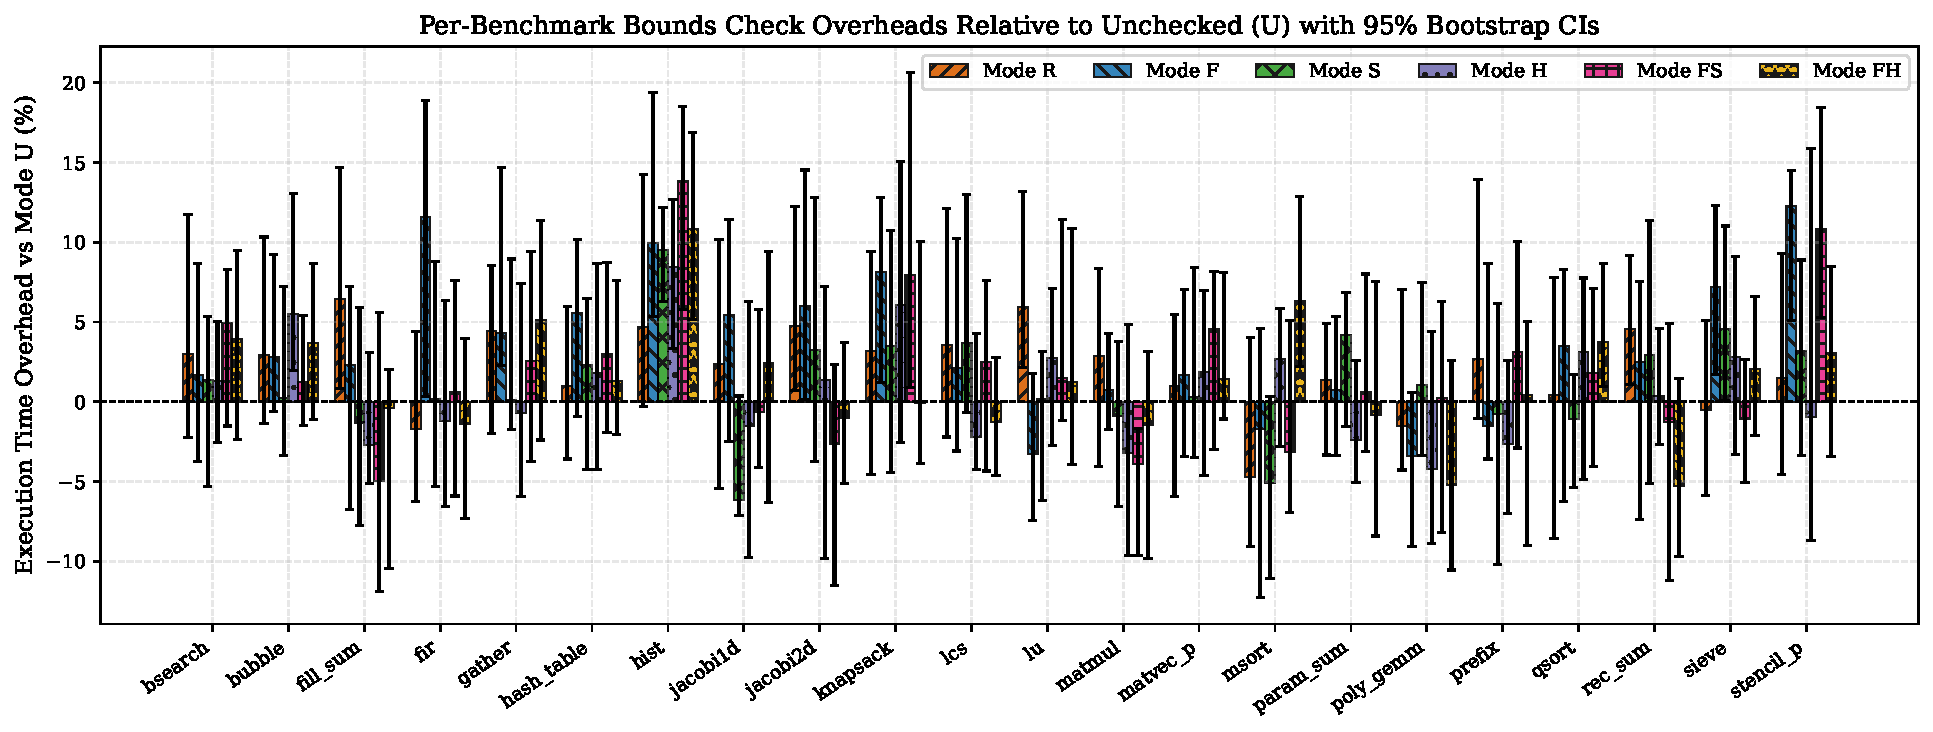
\includegraphics[width=0.95\linewidth]{overhead_bars.pdf}
\caption{Execution-time overhead relative to unchecked execution (U), with 95\% bootstrap intervals over 25 paired rounds.}\label{fig:overhead}
\end{figure}

\begin{table}[t]
\centering
\caption{Per-benchmark time overhead relative to U (median of paired ratios).}\label{tab:timing}
\small
% Auto-generated by scripts/generate_tables.py
\begin{tabular}{lrrrrrr}
\toprule
Benchmark & Mode R (\%) & Mode F (\%) & Mode S (\%) & Mode H (\%) & Mode FS (\%) & Mode FH (\%) \\
\midrule
bsearch & +3.00 & +1.69 & +1.37 & +1.31 & +4.92 & +3.92 \\
bubble & +2.91 & +2.82 & +0.25 & +5.52 & +1.24 & +3.67 \\
fib & -2.75 & -1.76 & -1.00 & -3.87 & -1.54 & -3.72 \\
fill\_sum & +6.44 & +2.33 & -1.30 & -2.72 & -4.94 & -0.39 \\
fir & -1.69 & +11.57 & +0.20 & -1.23 & +0.64 & -1.42 \\
gather & +4.45 & +4.31 & +0.14 & -0.73 & +2.57 & +5.15 \\
hash\_table & +1.01 & +5.59 & +2.28 & +1.80 & +2.97 & +1.30 \\
hist & +4.67 & +9.96 & +9.50 & +8.45 & +13.85 & +10.82 \\
jacobi1d & +2.39 & +5.42 & -6.19 & -1.54 & -0.62 & +2.43 \\
jacobi2d & +4.74 & +6.01 & +3.27 & +1.35 & -2.62 & -1.00 \\
knapsack & +3.21 & +8.13 & +3.51 & +6.07 & +7.96 & -0.08 \\
lcs & +3.53 & +2.14 & +3.71 & -2.22 & +2.49 & -1.24 \\
lu & +5.97 & -3.29 & +0.15 & +2.73 & +1.46 & +1.26 \\
matmul & +2.85 & +0.73 & -0.89 & -3.24 & -3.89 & -1.45 \\
matvec\_p & +1.00 & +1.65 & +0.30 & +1.88 & +4.58 & +1.41 \\
msort & -4.70 & -1.72 & -5.09 & +2.70 & -3.18 & +6.32 \\
param\_sum & +1.37 & +0.72 & +4.19 & -2.39 & +0.61 & -0.84 \\
poly\_gemm & -1.53 & -3.42 & +1.07 & -4.20 & +0.26 & -5.24 \\
prefix & +2.66 & -1.52 & -0.78 & -2.63 & +3.11 & +0.43 \\
qsort & +0.44 & +3.52 & -1.08 & +3.09 & +1.78 & +3.73 \\
rec\_sum & +4.55 & +2.51 & +2.93 & +0.34 & -1.29 & -5.26 \\
sieve & -0.54 & +7.18 & +4.58 & +2.80 & -1.06 & +2.03 \\
stencil\_p & +1.50 & +12.30 & +3.15 & -0.93 & +10.80 & +3.05 \\
\midrule
\textbf{Geomean (excl. fib)} & \textbf{+2.16} & \textbf{+3.49} & \textbf{+1.10} & \textbf{+0.69} & \textbf{+1.80} & \textbf{+1.24} \\
\bottomrule
\end{tabular}

\end{table}

\begin{figure}[t]
\centering
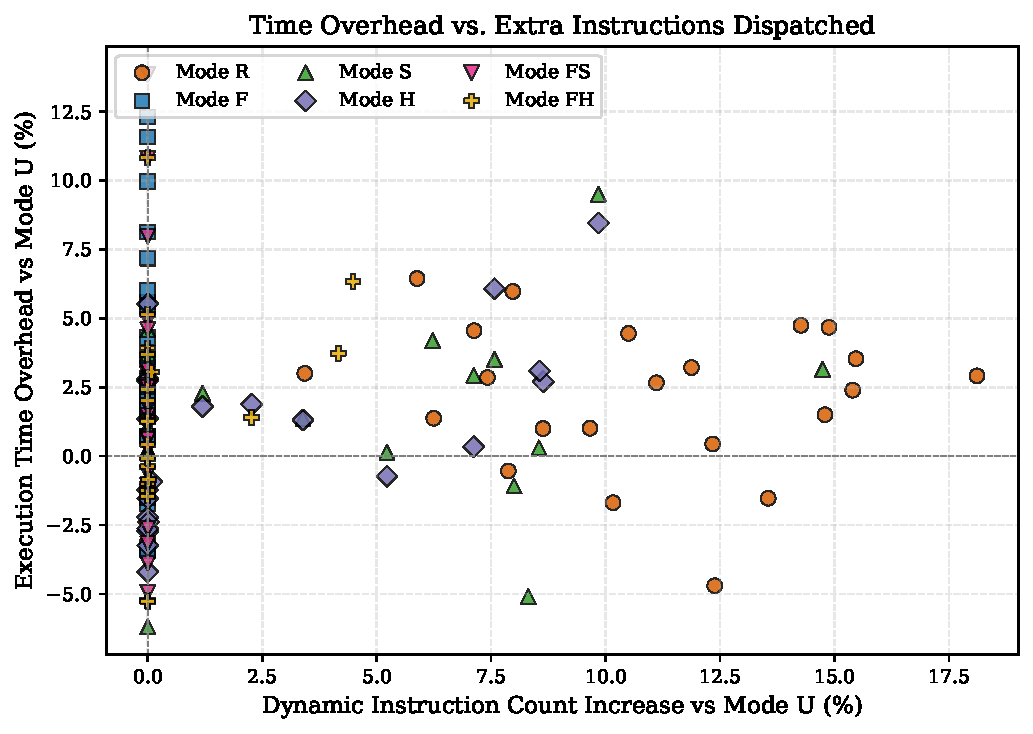
\includegraphics[width=0.8\linewidth]{scatter_overhead_instructions.pdf}
\caption{Time overhead versus extra instructions dispatched.}\label{fig:scatter}
\end{figure}

\subsection{RQ2: Dispatch versus comparison, and the role of dispatch technique}
Table~\ref{tab:dispatch} and Figure~\ref{fig:dispatch} compare dispatch implementations. With computed goto, N (an extra dispatch with no comparison) costs $+1.41\%$ against $+2.91\%$ for R in the same experiment, so dispatch alone accounts for about $48.5\%$ of the separate-check cost. With \texttt{switch} dispatch, N costs $+4.42\%$ against $+5.32\%$ for R, i.e.\ about $83.1\%$ of the cost is dispatch. With direct threading the overhead of R shrinks to $+0.32\%$, which is below our noise floor. The cost of a separate check therefore depends strongly on how the VM dispatches: the more expensive an extra dispatch is, the larger the share of the check cost it explains. (The R figures in this experiment differ slightly from those in Section~5.1 because they come from a separate run of the decomposition harness; see \texttt{results/dispatch\_ablation\_summary.csv}.)

\begin{table}[t]
\centering
\caption{Decomposition and dispatch ablation: geometric-mean overhead relative to U for each mode and dispatch technique.}\label{tab:dispatch}
\small
% Auto-generated by scripts/generate_tables.py
\begin{tabular}{lrrrrrrrr}
\toprule
Dispatch Technique & R (\%) & F (\%) & S (\%) & H (\%) & FS (\%) & FH (\%) & N (\%) & FN (\%) \\
\midrule
Computed GOTO (-O2) & +2.91 & +6.54 & +0.63 & +1.00 & +4.33 & +3.68 & +1.41 & +0.04 \\
Switch Dispatch (-O2) & +5.32 & -2.41 & +1.05 & +0.07 & +0.69 & -0.15 & +4.42 & -1.98 \\
Direct-Threaded (-O2) & +0.32 & +6.02 & +3.73 & +3.21 & +3.13 & +1.77 & +1.08 & +2.22 \\
Computed GOTO (-O3) & +3.47 & +2.97 & +2.72 & +2.50 & +3.53 & +4.21 & +1.51 & +0.62 \\
\bottomrule
\end{tabular}

\end{table}

\begin{figure}[t]
\centering
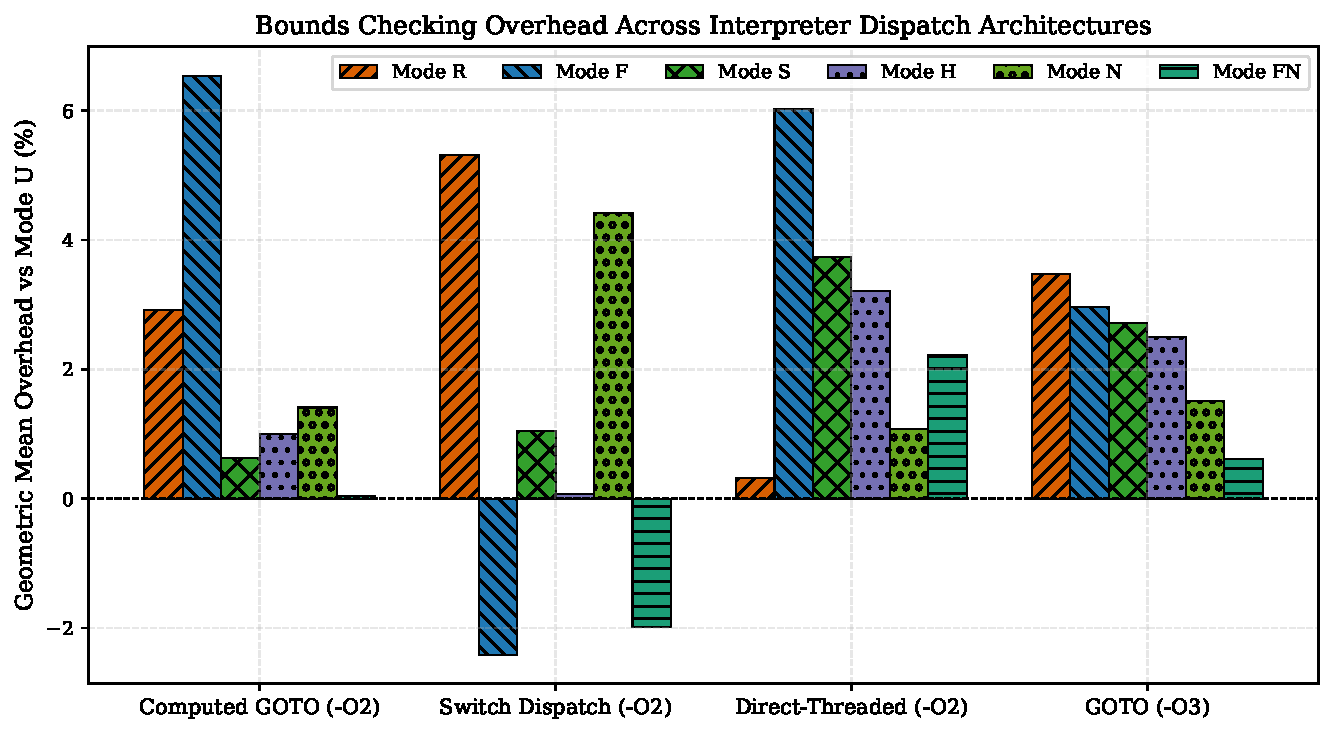
\includegraphics[width=0.95\linewidth]{dispatch_ablation.pdf}
\caption{Overhead of each mode under each dispatch technique.}\label{fig:dispatch}
\end{figure}

\begin{figure}[t]
\centering
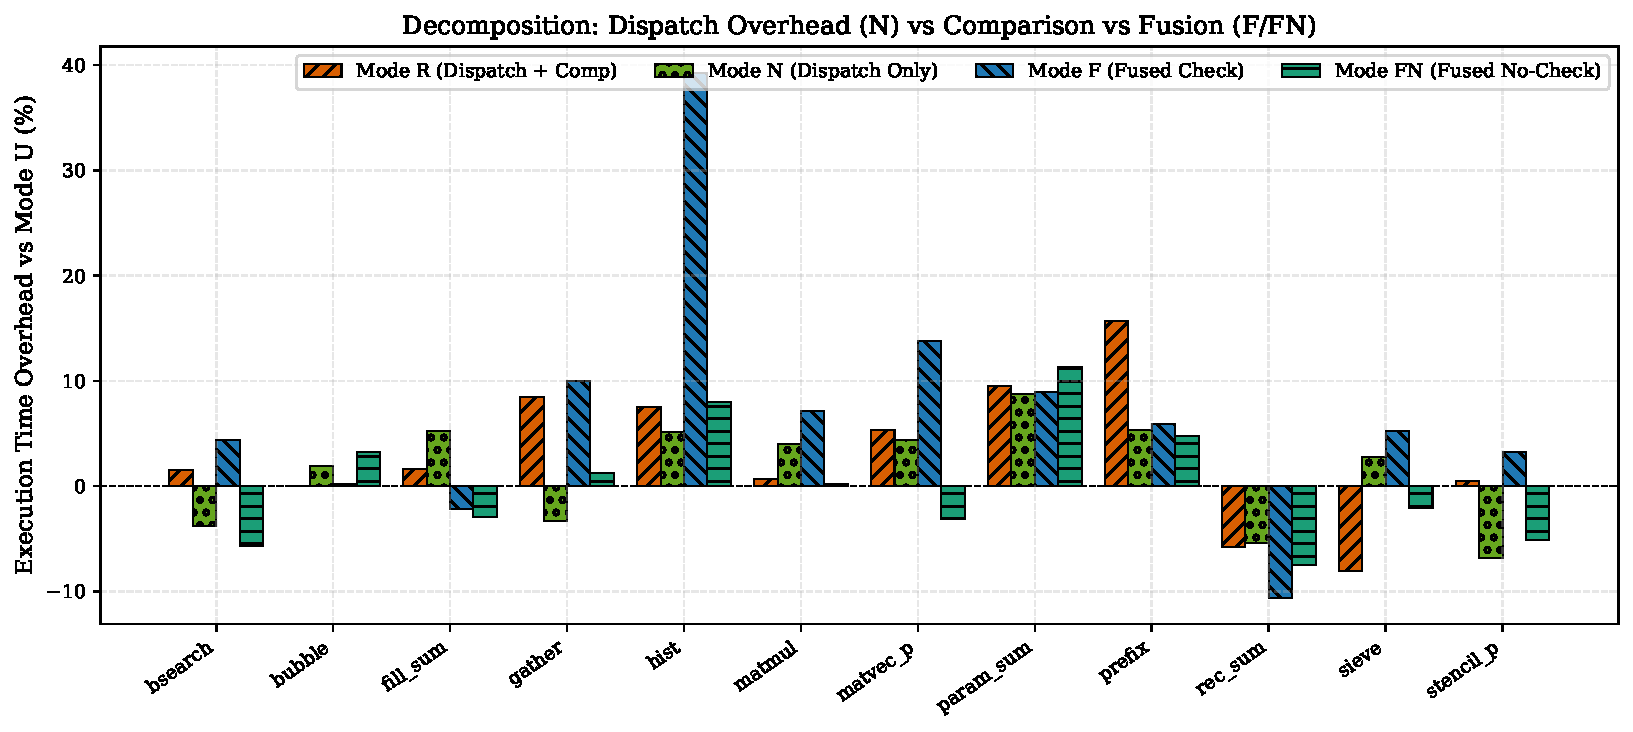
\includegraphics[width=0.85\linewidth]{decomposition.pdf}
\caption{Decomposition of check cost into extra dispatch (N), comparison with extra dispatch (R), fused comparison (F) and fused opcode without comparison (FN).}\label{fig:decomp}
\end{figure}

\paragraph{Fusion is not uniformly beneficial.} The naive expectation, that fusing the check into the access opcode removes the dispatch cost and hence nearly all overhead, holds only under \texttt{switch} dispatch, where F gives $-2.41\%$. Under computed goto, F is \emph{slower} than R ($+3.49\%$ vs.\ $+2.16\%$). The FN mode, which has the fused opcode but no comparison, is included to separate the effect of the opcode from the effect of the comparison (Table~\ref{tab:dispatch}). A plausible explanation is that the larger fused handlers worsen instruction-cache or code-layout behaviour, but we did not measure this and regard it as a hypothesis; since $+3.49\%$ and $+2.16\%$ differ by little more than the noise level, the sign of this effect should be confirmed on other hardware.

\subsection{RQ3: Static and dynamic check elimination}
Over the array benchmarks there are 104 access sites; interval analysis and hoisting remove checks at 81 of them ($77.9\%$), and the remainder stay as runtime checks (Table~\ref{tab:static}, Figure~\ref{fig:static}). Static counts understate the benefit because proved sites tend to lie in hot loops: dynamically, hoisting removes $88.5\%$ of the checks executed by R ($30.7$\,M checks; Table~\ref{tab:dynamic}, Figure~\ref{fig:dynamic}).

\begin{table}[t]
\centering
\caption{Static access-site classification per benchmark.}\label{tab:static}
\small
% Auto-generated by scripts/generate_tables.py
\begin{tabular}{lrrrrr}
\toprule
Benchmark & Total Sites & Safe (Mode S) & Hoisted (Mode H) & Residual (H) & Elim. Rate (\%) \\
\midrule
bsearch & 2 & 1 & 0 & 1 & 50.0\% \\
bubble & 10 & 10 & 0 & 0 & 100.0\% \\
fib & 0 & 0 & 0 & 0 & 0.0\% \\
fill\_sum & 2 & 2 & 0 & 0 & 100.0\% \\
fir & 7 & 7 & 0 & 0 & 100.0\% \\
gather & 4 & 3 & 0 & 1 & 75.0\% \\
hash\_table & 9 & 8 & 0 & 1 & 88.9\% \\
hist & 8 & 6 & 0 & 2 & 75.0\% \\
jacobi1d & 11 & 11 & 0 & 0 & 100.0\% \\
jacobi2d & 15 & 15 & 0 & 0 & 100.0\% \\
knapsack & 9 & 7 & 0 & 2 & 77.8\% \\
lcs & 15 & 15 & 0 & 0 & 100.0\% \\
lu & 16 & 16 & 0 & 0 & 100.0\% \\
matmul & 9 & 9 & 0 & 0 & 100.0\% \\
matvec\_p & 6 & 4 & 2 & 0 & 100.0\% \\
msort & 14 & 4 & 2 & 8 & 42.9\% \\
param\_sum & 2 & 1 & 1 & 0 & 100.0\% \\
poly\_gemm & 10 & 10 & 0 & 0 & 100.0\% \\
prefix & 7 & 7 & 0 & 0 & 100.0\% \\
qsort & 12 & 3 & 2 & 7 & 41.7\% \\
rec\_sum & 2 & 1 & 0 & 1 & 50.0\% \\
sieve & 6 & 6 & 0 & 0 & 100.0\% \\
stencil\_p & 8 & 4 & 4 & 0 & 100.0\% \\
\midrule
\textbf{Total} & \textbf{184} & \textbf{150} & \textbf{11} & \textbf{23} & \textbf{87.5\%} \\
\bottomrule
\end{tabular}

\end{table}

\begin{figure}[t]
\centering
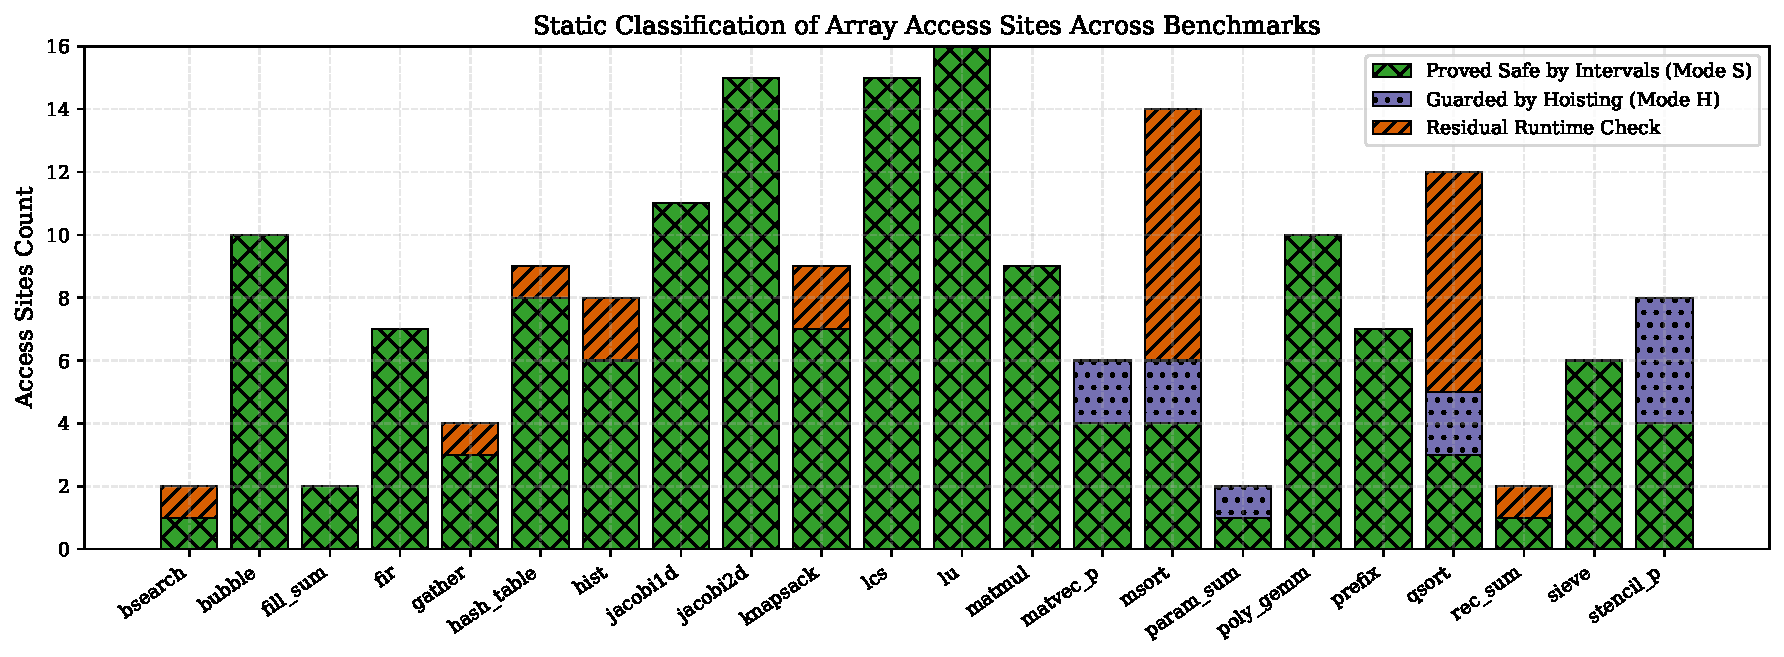
\includegraphics[width=0.9\linewidth]{static_classification.pdf}
\caption{Static classification of access sites: proved safe by intervals, guarded by hoisting, residual runtime check.}\label{fig:static}
\end{figure}

\begin{table}[t]
\centering
\caption{Dynamic checks executed per mode.}\label{tab:dynamic}
\small
% Auto-generated by scripts/generate_tables.py
\begin{tabular}{lrrrrr}
\toprule
Benchmark & Checks (Mode R) & Checks (Mode S) & Checks (Mode H) & Checks (Mode FH) & Elim. (FH vs R) \\
\midrule
bsearch & 349,147 & 345,051 & 345,051 & 345,051 & 1.2\% \\
bubble & 2,996,012 & 0 & 0 & 0 & 100.0\% \\
fib & 0 & 0 & 0 & 0 & 0.0\% \\
fill\_sum & 800,000 & 0 & 0 & 0 & 100.0\% \\
fir & 2,037,952 & 0 & 0 & 0 & 100.0\% \\
gather & 1,646,592 & 819,200 & 819,200 & 819,200 & 50.2\% \\
hash\_table & 403,610 & 50,000 & 50,000 & 50,000 & 87.6\% \\
hist & 1,857,346 & 1,228,800 & 1,228,800 & 1,228,800 & 33.8\% \\
jacobi1d & 3,319,840 & 0 & 0 & 0 & 100.0\% \\
jacobi2d & 1,714,080 & 0 & 0 & 0 & 100.0\% \\
knapsack & 1,251,897 & 798,210 & 798,210 & 798,210 & 36.2\% \\
lcs & 3,415,357 & 0 & 0 & 0 & 100.0\% \\
lu & 731,750 & 0 & 0 & 0 & 100.0\% \\
matmul & 1,740,875 & 0 & 0 & 0 & 100.0\% \\
matvec\_p & 1,655,560 & 1,638,400 & 0 & 0 & 100.0\% \\
msort & 1,243,034 & 834,464 & 417,232 & 417,232 & 66.4\% \\
param\_sum & 1,255,000 & 1,250,000 & 0 & 0 & 100.0\% \\
poly\_gemm & 2,086,400 & 0 & 0 & 0 & 100.0\% \\
prefix & 1,600,000 & 0 & 0 & 0 & 100.0\% \\
qsort & 771,366 & 500,259 & 275,127 & 275,127 & 64.3\% \\
rec\_sum & 801,000 & 800,000 & 800,000 & 800,000 & 0.1\% \\
sieve & 1,473,950 & 0 & 0 & 0 & 100.0\% \\
stencil\_p & 1,805,100 & 1,798,800 & 0 & 0 & 100.0\% \\
\midrule
\textbf{Total} & \textbf{34,955,868} & \textbf{10,063,184} & \textbf{4,733,620} & \textbf{4,733,620} & \textbf{86.5\%} \\
\bottomrule
\end{tabular}

\end{table}

\begin{figure}[t]
\centering
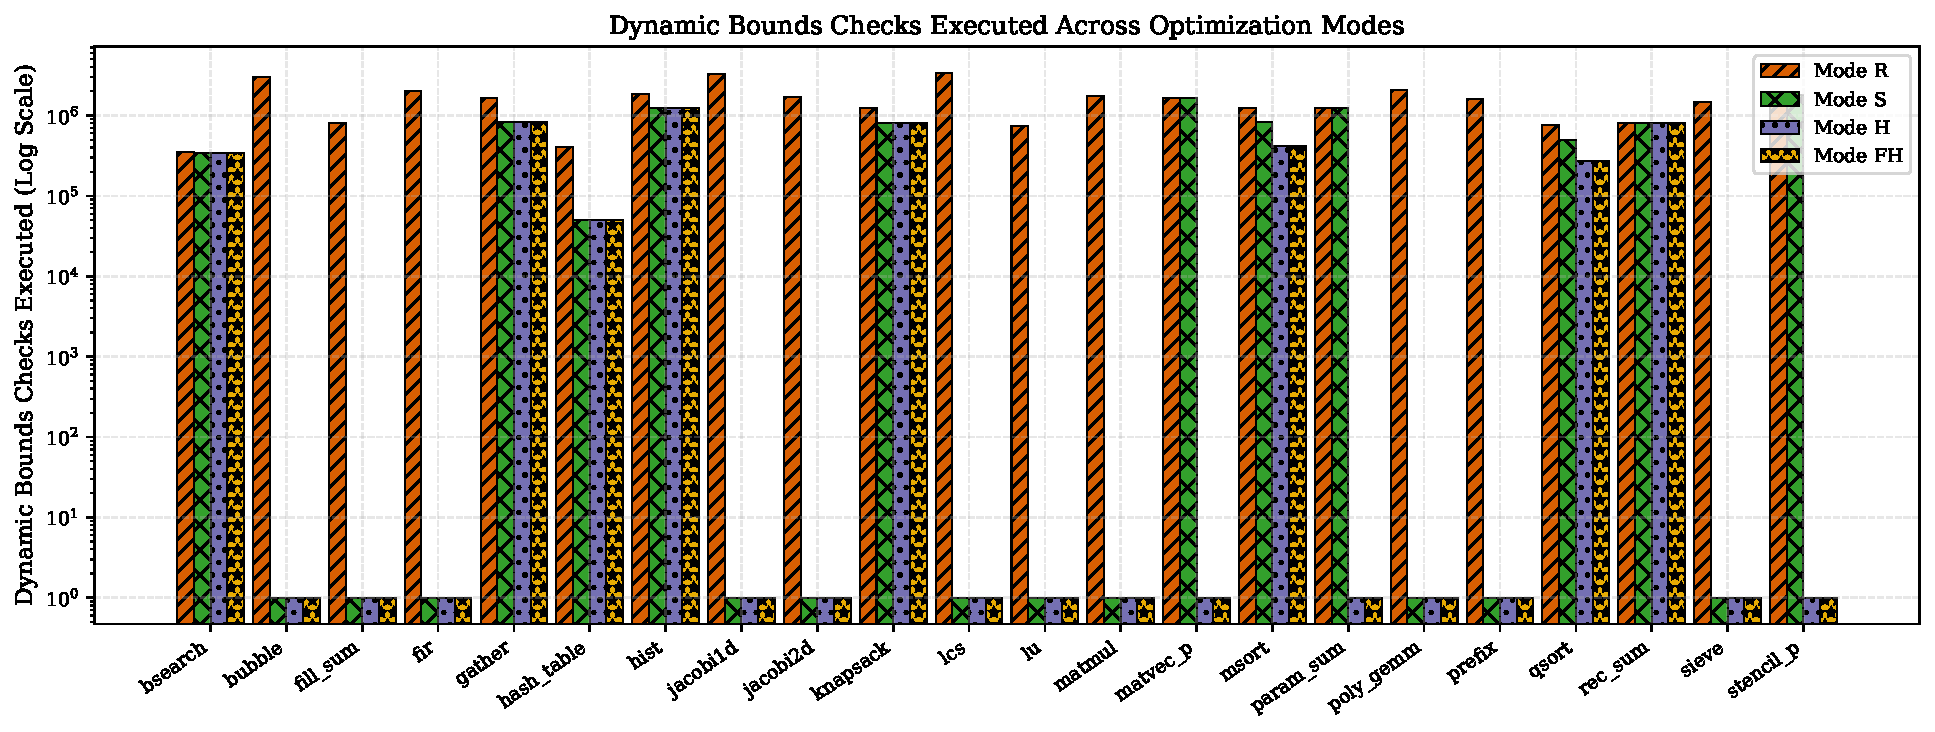
\includegraphics[width=0.9\linewidth]{dynamic_checks.pdf}
\caption{Dynamic checks executed by S and H as a percentage of those executed by R.}\label{fig:dynamic}
\end{figure}

In time (computed goto, 22 array benchmarks), S reduces the overhead from $+2.16\%$ to $+1.10\%$ and H to $+0.69\%$, recovering roughly two thirds of R's overhead; H brings the overhead below the level we can distinguish from the noise floor. For the original 12 benchmarks the corresponding values are $+2.89\%$ (R), $+1.91\%$ (S) and $+0.58\%$ (H). The combined modes give $+1.80\%$ (FS) and $+1.24\%$ (FH). Hoisting is useful precisely where interval analysis fails on a parameter-bounded loop (\texttt{param\_sum}, \texttt{stencil\_p}, \texttt{matvec\_p}), and adds nothing on benchmarks whose indices are loaded data or recursion parameters (\texttt{gather}, \texttt{hist}, \texttt{rec\_sum}). Hoisting costs code size (\todo{insert bytecode size growth per mode from results/ CSV}).

\paragraph{Two-tier view.} H leaves a small residue of checks that neither analysis nor hoisting can remove. FH implements the combination of both tiers, hoisting for what can be guarded and fused checks for the rest. In our measurements, FH ($+1.24\%$) is not better than H ($+0.69\%$) under computed goto, consistent with fusion not helping under that dispatch, so the two-tier design is attractive mainly for dispatch styles in which fusion pays off.

\subsection{RQ4: Residual checks and fault injection}
The sites that remain as runtime checks fall into three classes. (i) \emph{Data-dependent indices}: values loaded from memory are $\top$ in a non-relational domain (\texttt{gather}, \texttt{hist}). (ii) \emph{Recursion parameters}, since the analysis is intraprocedural (\texttt{rec\_sum}). (iii) \emph{Non-innermost parameter loops}, since we version innermost loops only. Classes (ii) and (iii) are limits of our implementation, whereas (i) requires relational or value-set reasoning and is inherently limited when data come from the environment.

Table~\ref{tab:fault} and Figure~\ref{fig:fault} summarise fault injection. Of the faulty mutants (those on which R traps), 213 in total, $195$ ($91.5\%$) are noticed by static analysis, as either a definite violation or strictly more non-proved sites than the original program. Off-by-one style faults typically make the index interval straddle the array bound rather than lie wholly outside it, so definite violations are rare and most detections are alarms. Under U, none of the faulty mutants crashed, and $181$ of the $213$ ($85.0\%$) ran to completion silently; this is the safety gap that motivates checking at all. Differential testing across R, F, S, H, FS and FH found \todo{state exactly: no divergences, per results/fault\_injection\_summary.json}.

\begin{table}[t]
\centering
\caption{Fault-injection outcomes by mutation operator.}\label{tab:fault}
\small
% Auto-generated by scripts/generate_tables.py
\begin{tabular}{lrrrrrr}
\toprule
Mutation Operator & Mutants & Faulty (Trapped) & Benign & Compile-time Viol. & Static Alarms & Silent U Corrupt. \\
\midrule
cond_lt_to_le & 51 & 30 & 21 & 0 & 27 & 21 \\
index_minus_1 & 43 & 33 & 10 & 0 & 30 & 35 \\
index_minus_k & 43 & 41 & 2 & 0 & 32 & 37 \\
index_plus_1 & 43 & 32 & 11 & 0 & 31 & 35 \\
index_plus_k & 43 & 34 & 9 & 0 & 32 & 36 \\
missing_loop_update & 58 & 0 & 58 & 0 & 0 & 2 \\
swapped_loop_vars & 2 & 0 & 2 & 0 & 0 & 1 \\
wrong_array_bound & 46 & 43 & 3 & 5 & 38 & 14 \\
\midrule
\textbf{Total} & \textbf{329} & \textbf{213} & \textbf{116} & \textbf{5} & \textbf{190} & \textbf{181} \\
\bottomrule
\end{tabular}

\end{table}

\begin{figure}[t]
\centering
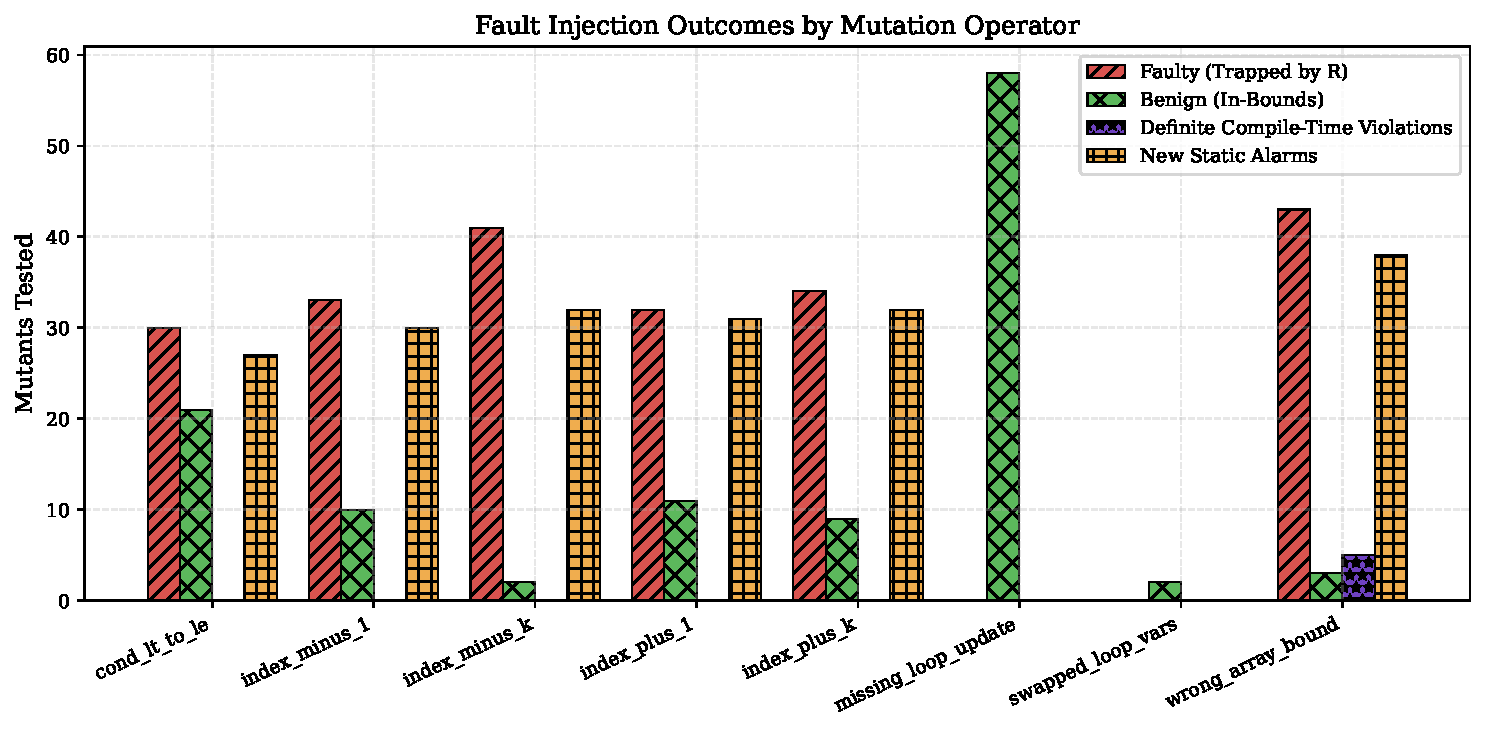
\includegraphics[width=0.9\linewidth]{fault_injection_bars.pdf}
\caption{Outcome of injected faults by mutation operator.}\label{fig:fault}
\end{figure}

%--------------------------------------------------------------------
\section{Discussion}
\paragraph{What the results say.} In this interpreter, bounds checking is cheap: $2$--$3\%$ under computed goto. The cost of the check is not fixed, however; it moves with the dispatch technique, from over $5\%$ under \texttt{switch} to well under $1\%$ with direct threading. The decomposition shows that the extra dispatch explains a substantial part of that cost, roughly half under computed goto and most of it under \texttt{switch}, which supports the view that encoding choices matter in interpreters in a way they do not in native code.

\paragraph{Design implications.} (1) If a VM must use a \texttt{switch} loop, fuse checks into accesses. (2) If it uses computed goto or direct threading, separate checks are already inexpensive and fusion is not worth the extra handlers; eliminating checks by analysis gives the larger and more portable gain. (3) Loop-guard hoisting recovers most of the remaining cost without any change to the VM, which is valuable where the VM is part of a trusted computing base that is hard to change or audit. Static elimination also remains valuable for diagnostics, independent of speed.

\paragraph{Relation to expectations.} Before the experiments we expected overheads near $10\%$ and fusion to be close to free. The measurements contradict both expectations, which is why we report the dependence on dispatch technique rather than a single number.

%--------------------------------------------------------------------
\section{Threats to Validity and Limitations}\label{sec:threats}
\paragraph{Internal validity.} Timing is on a single virtualised machine (WSL2) with a noise floor comparable to several of the effects we report; CIs for individual benchmarks often overlap, and differences below the noise level, including between H and U, are not supported. Hardware counters (\texttt{perf stat}) are not available under WSL2; we use user-space \texttt{rdtsc} cycles, which are not a substitute for branch-misprediction and IPC data, so we cannot attribute the dispatch costs to specific microarchitectural events. Interval soundness assumes no integer wrap-around, and the hoisting argument is a proof sketch supported by differential and randomized testing, not a mechanised proof. The Windows validation scripts are provided but results from them are not part of this paper.

\paragraph{External validity.} The benchmark programs are small and hand-written (23 programs), the language has only global fixed-size arrays, and the VM is a simple interpreter; a JIT, registers, or heap objects with dynamic lengths would change both the costs and the analysis. Results come from one CPU model and one compiler version. Mutants are synthetic faults, not field bug data.

\paragraph{Novelty scope.} Range-check hoisting by loop versioning is known in optimizing compilers~\cite{midkiff1998,gupta1993}, and superinstructions are well established~\cite{proebsting1995}. Our contribution is the controlled measurement across encodings and dispatch techniques, with the dispatch/comparison decomposition, and the expression of the guard in the existing ISA. We have not performed an exhaustive literature or patent search.

%--------------------------------------------------------------------
\section{Conclusion and Future Work}
In a bytecode interpreter the overhead of bounds checking depends on how checks are encoded and how the VM dispatches. Under computed goto it is about $2$--$3\%$ on our benchmarks, roughly half of which is the dispatch of the extra check instruction; under \texttt{switch} dispatch the cost is higher and mostly dispatch, and fusing the check helps; with direct threading the cost nearly vanishes. Interval analysis plus ISA-preserving loop-guard hoisting removes $88.5\%$ of dynamic checks and reduces overhead to $+0.69\%$ without changing the VM, and fault injection shows that most injected off-by-$k$ faults are visible to the analysis as alarms even though few are definite violations. Future work includes microarchitectural counters on native Linux, ARM64 and other CPUs, relational domains, interprocedural summaries, hoisting for non-innermost and descending loops, register-based VMs, JIT back-ends and larger benchmark suites.

\section*{Data and Code Availability}
The complete toolchain, benchmarks, raw results and scripts are available in a repository accompanying this paper (\texttt{minil-bounds-vm}); \todo{insert public or archived link, if allowed}.

\begin{thebibliography}{99}\small
\bibitem{haas2017} A. Haas et al., ``Bringing the web up to speed with WebAssembly,'' in \emph{Proc. PLDI}, 2017, pp. 185--200.
\bibitem{jangda2019} A. Jangda, B. Powers, E. D. Berger, and A. Guha, ``Not so fast: Analyzing the performance of WebAssembly vs.\ native code,'' in \emph{Proc. USENIX ATC}, 2019, pp. 107--120.
\bibitem{nagarakatte2009} S. Nagarakatte, J. Zhao, M. M. K. Martin, and S. Zdancewic, ``SoftBound: Highly compatible and complete spatial memory safety for C,'' in \emph{Proc. PLDI}, 2009, pp. 245--258.
\bibitem{serebryany2012} K. Serebryany, D. Bruening, A. Potapenko, and D. Vyukov, ``AddressSanitizer: A fast address sanity checker,'' in \emph{Proc. USENIX ATC}, 2012, pp. 309--318.
\bibitem{akritidis2009} P. Akritidis, M. Costa, M. Castro, and S. Hand, ``Baggy bounds checking: An efficient and backwards-compatible defense against out-of-bounds errors,'' in \emph{Proc. USENIX Security}, 2009, pp. 51--66.
\bibitem{necula2005} G. C. Necula, J. Condit, M. Harren, S. McPeak, and W. Weimer, ``CCured: Type-safe retrofitting of legacy software,'' \emph{ACM TOPLAS}, vol. 27, no. 3, pp. 477--526, 2005.
\bibitem{jones1997} R. W. M. Jones and P. H. J. Kelly, ``Backwards-compatible bounds checking for arrays and pointers in C programs,'' in \emph{Proc. AADEBUG}, 1997, pp. 13--26.
\bibitem{suzuki1977} N. Suzuki and K. Ishihata, ``Implementation of an array bound checker,'' in \emph{Proc. POPL}, 1977, pp. 132--143.
\bibitem{gupta1993} R. Gupta, ``Optimizing array bound checks using flow analysis,'' \emph{ACM Letters on Programming Languages and Systems}, 1993. \todo{verify volume and pages}
\bibitem{kolte1995} P. Kolte and M. Wolfe, ``Elimination of redundant array subscript range checks,'' in \emph{Proc. PLDI}, 1995, pp. 270--278.
\bibitem{bodik2000} R. Bod\'ik, R. Gupta, and V. Sarkar, ``ABCD: Eliminating array bounds checks on demand,'' in \emph{Proc. PLDI}, 2000, pp. 321--333.
\bibitem{midkiff1998} S. P. Midkiff, J. E. Moreira, and M. Snir, ``Optimizing array reference checking in Java programs,'' \emph{IBM Systems Journal}, vol. 37, no. 3, pp. 409--453, 1998.
\bibitem{wurthinger2009} T. W\"urthinger, C. Wimmer, and H. M\"ossenb\"ock, ``Array bounds check elimination in the context of deoptimization,'' \emph{Science of Computer Programming}, vol. 74, no. 5--6, pp. 279--295, 2009.
\bibitem{proebsting1995} T. A. Proebsting, ``Optimizing an ANSI C interpreter with superoperators,'' in \emph{Proc. POPL}, 1995.
\bibitem{ertl2003} M. A. Ertl and D. Gregg, ``Optimizing indirect branch prediction accuracy in virtual machine interpreters,'' in \emph{Proc. PLDI}, 2003.
\bibitem{casey2007} K. Casey, M. A. Ertl, and D. Gregg, ``Optimizing indirect branch prediction accuracy in virtual machine interpreters,'' \emph{ACM TOPLAS}, 2007. \todo{verify pages}
\bibitem{rohou2015} E. Rohou, B. N. Swamy, and A. Seznec, ``Branch prediction and the performance of interpreters: Don't trust folklore,'' in \emph{Proc. CGO}, 2015, pp. 103--114.
\bibitem{ertl2024} M. A. Ertl and B. Paysan, ``The performance effects of virtual-machine instruction pointer updates,'' in \emph{Proc. ECOOP}, 2024, pp. 14:1--14:26.
\bibitem{shi2008} Y. Shi, K. Casey, M. A. Ertl, and D. Gregg, ``Virtual machine showdown: Stack versus registers,'' \emph{ACM TACO}, vol. 4, no. 4, article 2, 2008.
\bibitem{vishwanathan2023} H. Vishwanathan, M. Shachnai, S. Narayana, and S. Nagarakatte, ``Verifying the verifier: eBPF range analysis verification,'' in \emph{Proc. CAV}, 2023, pp. 226--251.
\bibitem{cousot1977} P. Cousot and R. Cousot, ``Abstract interpretation: A unified lattice model for static analysis of programs by construction or approximation of fixpoints,'' in \emph{Proc. POPL}, 1977, pp. 238--252.
\bibitem{cousot1978} P. Cousot and N. Halbwachs, ``Automatic discovery of linear restraints among variables of a program,'' in \emph{Proc. POPL}, 1978, pp. 84--96.
\bibitem{mine2006} A. Min\'e, ``The octagon abstract domain,'' \emph{Higher-Order and Symbolic Computation}, vol. 19, no. 1, pp. 31--100, 2006.
\bibitem{leroy2009} X. Leroy, ``Formal verification of a realistic compiler,'' \emph{Communications of the ACM}, vol. 52, no. 7, pp. 107--115, 2009.
\end{thebibliography}

\end{document}
